\documentclass[12pt,a4paper]{article}
\usepackage[margin=20mm, includefoot, heightrounded]{geometry}
\usepackage{indentfirst}
\usepackage{subcaption}
\usepackage{varwidth}
\usepackage[noend]{algpseudocode}
\usepackage{algorithm}
\usepackage{enumitem}
\usepackage{graphicx}
\usepackage{multicol}
\usepackage{mathtools}
\usepackage[labelfont=bf]{caption} % Required for specifying captions to tables and figures
\usepackage{amsmath}

\setenumerate{leftmargin=*, itemsep=1em, topsep=1em}
\setlist{parsep=0pt,listparindent=\parindent} % Used for the blank space in the head of paragraphes

\renewcommand{\algorithmicrequire}{\textbf{Input:}}  % Turn Require into Input
\renewcommand{\algorithmicensure}{\textbf{Output:}} % Turn Ensure into Output

\title{
	{\bf CSE505 - Computing with Logic
	\\\vspace{1em}
	A New Algorithm to Automate Inductive Learning of Default Theories}
}
\author{
	FARHAD SHAKERIN, ELMER SALAZAR, GOPAL GUPTA\\
	\vspace{1em}
	ICLP, August 2017\\
	Wei-Cheng Li\\
	112073486
}
\date{December 17, 2018}
\begin{document}
	\maketitle
	
	\begin{section}{Introduction}
	In an inductive learning programming (ILP) process, the program learns theories from the positive and negative examples and discovers the corresponding rules. However, the typical ILP systems treat the exceptions and the noise in the same way. ILP cannot handle the exceptions whereas they sometimes follow a pattern which can also be learned to a general rule. For example, we want to learn the concept of birds’ flying ability. We know that in most cases birds can fly, but there are some birds such as penguins and ostriches that are the exceptions. Here, ILP systems will either fail to determine a general rule or cover the positive examples without caring much about negative ones. Other algorithms, such as First Order Inductive Learning (FOIL), induces rules that are non-constructive, thus it is sometimes not intuitive at all.

	To tackle this problem, the authors introduced new algorithms, which are the extension of FOIL, called First Order Learner of Default (FOLD)\cite{FOLD} and FOLD-R to handle categorical and numeric features respectively. Both of them learn non-monotonic stratified logic program which allows negation-as-failure (NAF).
	\end{section}

	\begin{section}{Background}
		\begin{subsection}{Problem Statement}
			We follow the statements provided in the paper. For an inductive non-monotonic logic programming problem, it can be formalized as below:\\
			
			\noindent {\bf Given}
			\begin{itemize}
				\item {a background theory $B$ in the form of a normal logic program, i.e. clauses of the form $h\leftarrow l_1, ... l_m$, $\neg l_{m+1},...,\neg l_n$, where $l_1,...,l_n$ are positive literals.}
				\item {two disjoint seets of grounded goal predicates $E+$ and $E-$ as positive examples and negative examples respectively.}
				\item {a function $covers(H,E,B)$ that returns the subset of $E$ which is implied by the hypothesis $H$ given the background knowledge $B$.}
				\item {a function $score(E+,E-,H,B)$ that specifies the quality of the hypothesis $H$ with respect to $E+$, $E-$, $B$.}
			\end{itemize}
			\noindent {\bf Objective}
				\begin{itemize}
					\item {find a theory $T$ that makes $covers(T,E+,B)=E+$ and $covers(T,E-,B)=\phi$}
				\end{itemize}

			Namely, we want to find a set of rules, which satisfies all of the positive examples and rules out all of the negative examples.
		\end{subsection}

		\begin{subsection}{FOIL Algorithm}
		The FOLD algorithm is an extension of the FOIL algorithm (Quinlan 1990). The FOIL algorithm is a top-down ILP system following a sequential covering approach to induce a hypothesis. The algorithm can be summarized as Algorithm 1. Basically, FOIL repeatedly searches for the clauses with the greatest score with respect to $E+$, $E-$, and the hypothesis $H$ at that time.
		\makebox[\linewidth]{
				\begin{minipage}{\dimexpr\linewidth}
				\begin{algorithm}[H]
				\caption{FOIL Algorithm Summary}
				\begin{algorithmic}[1]
					\Require{goal, $B$, $E+$, $E-$}
					\Ensure{theory $T$}
					\Function{FOIL}{goal, $B$, $E+$, $E-$}
					\State initialize $T \gets \phi$
					\While {$size(E+)>0$}
						\State $c\gets (goal \text{ :- } true.)$ 
						\While {$size(E-)>0$}
							\For {each candidate literal $l$}
								\State compute $score(E+,E-,H\cup\{c'\}, B)$
							\EndFor
							\State conjoin $l$ with the best score to $c.body$
							\State $E-\gets E-$\textbackslash{}$covers(\neg c, E-, B)$
						\EndWhile
						\State add $c$ to $T$
						\State $E+\gets E+$\textbackslash $covers(c,E+,B)$  
					\EndWhile
					\State\Return $T$
					\EndFunction
				\end{algorithmic}
				\end{algorithm}
				\end{minipage}
		}\\

		The score in line 7 is the information gain (IG) of the corresponding rule, which is calculated as follows (Mitchell 1997):
		\begin{gather*}
		\centering IG(L,R)=t(log_2{\frac{p_1}{p_1+n_1}}-log_2{\frac{p_0}{p_0+n_0}})
		\end{gather*}
		where $L$ is the candidate literal to conjoin to the body of the rule $R$, $p_0$ is the number of positive examples implied by $R$, $n_0$ is the number of negative examples implied by $R$, $p_1$ is the number of positive examples implied by $L+R$, $n_1$ is the number of negative examples implied by $L+R$, and $t$ is the number of positive examples implied by $R$ also covered by $R+L$.

		Basically, the clause with the "best" literal added increases the largest number of positive examples that satisfy the rule. Nevertheless, this approach cannot capture the exceptions and the result somtimes is not much intuitive for humans.
		\end{subsection}
	\end{section}

	\begin{section}{Method}
		Like the FOIL algorithm, the FOLD algorithm repeatedly explores new literal and conjoins it to the current rule theory. The difference is that, first, FOLD do not consider negative literals when exploring. Second, when there is no improvement with the remain literals, FOLD then tries to find the rules governing negative examples. This can be viewed as a subproblem by swappping the postive and negative examples, so we just call the FOLD algorithm recursively. The below steps shows the progress of how it works:
		\begin{enumerate}
			\item {
				The function $FOLD(goal,E+,E-,B)$ returns a set of rules that satisfies all $E+$ and rules out all $E-$, with the given background knowledges. The rule starts with the most general one, i.e., $goal$ :- $true.$

			}
			\item {
				For each iteration, FOLD picks the literal with maximum information gain. That is, we maintains the coverage as many positive examples as possible.
			}
			\item {
				Step 2 stops when the information gain is zero.
			}
			\item {
				If $|E-|$ is not zero, they are either noisy data or exceptions. Then, we try to find the rules governing the negative examples. This step is called $exception$ and can be done by calling $FOLD(goal, E-,E+,B)$ (step 1).
			}
			\item {
				In $exception$ step, when we find a rule for the exceptions, we create a new predicate and add the negation of it to the rule set.
			}
			\item {
				If no pattern can be learned due to the lack of information or the noisy data, FOLD then enumerates the rest positive examples.
			}
		\end{enumerate}
	\end{section}

	\begin{section}{Project Work}
		I implemented the FOLD algorithm with several functions in SWI-Prolog, and then test them 
		with several different types of cases.
		\begin{subsection}{Functions}
			\begin{enumerate}
				\item {
					{\bf fold (Goal, Pos, Neg, Background, Predicates, D, AB, IsExcept)}

					The main function of the algorithm. We start with {\bf Goal} $=goal\text{ :- }true$ and finally return the set of rules {\bf D} and {\bf AB}. {\bf D} denotes the default clauses while {\bf AB} denotes the abnormal clauses (exceptions). {\bf IsExcept} checks whether the current process is called in the exception step.

				}
				\item {
					{\bf fold\_loop (Goal, Pos, Neg, IsExcept, Prev, D)}

					This is the looping function which repeatedly calls the specialize function. It stops when {\bf Pos} is empty. Every time the specialize function returns a new clause, we append it to {\bf Prev}. Eventually, we assign {\bf D} to {\bf Prev} when the loop stops.
				}
				\item {
					{\bf specialize (Pos, Neg, Clause0, PosClause, Just\_started)}

					Find and return a rule as {\bf PosClause} based on positive examples ({\bf Pos}), negative examples ({\bf Neg}), hypothesis ({\bf Clause0}), and the background knowledge. {\bf Just\_started} checks if it is the first call to determine the next action (enumerate or exception) if we get IG=0.
				}
				\item {
					{\bf exception ((Goal :- Body), Pos, Neg, Clause1)}

					Call fold function to get the exception rules governing {\bf Neg}. After finding the rules, we create a new predicate and append it to {\bf Body}, becoming {\bf Clause1}. The predicate is also added to the abnormal clauses set.
				}
				\item {
					{\bf enumerate (Clause0, Pos, Clause1)}

					The function enumerates the positive clauses. We create a clause $member/2$ which is also the built-in function in Prolog to represent the enumerating process. We then add it to the body of {\bf Clause0} as {\bf Clause1}.
				}
				\item {
					{\bf compute\_gain (Neg, Pos, Info, Clause, Gain)}

					Return the IG value given {\bf Clause}, the examples {\bf Pos} and {\bf Neg}, and the gain value {\bf Info} representing IG without {\bf Clause} added to the rule.
				}
			\end{enumerate}
		\end{subsection}
		\begin{subsection}{Tools}
		There are some other functions to help the main functions manage the important tasks.
		\begin{enumerate}
			\item {
				{\bf unify\_arg(L, Head, Result)}

				To create a predicate, we have to make the variables consistent in both the head and the body. This function unifies the variable in literal {\bf L} and the one in the predicate's head {\bf Head}.
			}
			\item {
				{\bf add\_best\_literal(Clause0, Pos, Neg, Clause1, IG)}

				This function is used in the specialze function when we have to pick a best literal in every turn. Basically it calculate every litaral candidate with the compute\_gain/5 function, and return the greatest one with its {\bf IG}.
			}
			\item {
				{\bf choose\_tie\_clause(Clause, B0, B1, C)}

				If we find there are multiple literal candidates with the same information gain value, we choose the one with the least constraints. We append the literals {\bf B0} and {\bf B1} to {\bf Clause} respectively and pick up the one with less number of variables.
			}
			\item {
				{\bf covered\_examples((A:-B), Xs, Xs1)}

				This function acts as $covers(H,E,B)$. Given the predicate {\bf (A:-B)} and the example {\bf Xs}, we filter out the unsatisfied examples and return the rest as {\bf Xs1}.
			}
			\item {
				{\bf uncovered\_examples((A:-B), Xs, Xs1)}

				Similar with the above, but this time we filter out the satisfied elements and return the rest as {\bf Xs1}.
			}
		\end{enumerate}
		\end{subsection}
	\end{section}

	\begin{section}{Testing}
		To verify the algorithm, I used the testing data provided in the paper, each of which is designed under different conditions, including the noisy data and the exceptions. Moreover, I further used a more complicated dataset outside the paper to see if the algorithm can still achieve a high accuracy.
		\vspace{4em}
		\renewcommand{\arraystretch}{1.3}
		\begin{subsection}{Single Exception}
			\begin{multicols}{2}
				\noindent {\bf Input:} \vspace{-1em}
				\begin{table}[H]
					\begin{tabular}{rl}
					Background: & bird(X) $\leftarrow$ penguin(X). \\
					            & bird(tweety). bird(et).                       \\
					            & cat(kitty). penguin(polly).                   \\
					Example+:   & \{tweety, et\}                                \\
					Example-:   & \{kitty, polly\}                              \\
					Goal:       & fly(X)                                      
					\end{tabular}
				\end{table}
				\columnbreak
				\noindent {\bf Output:} \vspace{-1em}
				\begin{table}[H]
					\begin{tabular}{rl}
					D: & fly(X) $\leftarrow$ bird(X), \textbackslash{+ab0(X)}. \\
					AB:& ab0(X) $\leftarrow$ penguin(X).\\
					\end{tabular}
				\end{table}
			\end{multicols}
		\end{subsection}
		
		\begin{subsection}{Enumerate}
			\begin{multicols}{2}
			\noindent {\bf Input:} \vspace{-1em}
				\begin{table}[H]
					\begin{tabular}{rl}
					Background: & bird(X) $\leftarrow$ penguin(X). \\
					            & bird(tweety). bird(et).                       \\
					            & cat(kitty). penguin(polly).                   \\
					Example+:   & \{tweety, et, {\bf jet}\}                     \\
					Example-:   & \{kitty, polly\}                              \\
					Goal:       & fly(X)                                      
					\end{tabular}
				\end{table}
				\columnbreak
				\noindent {\bf Output:} \vspace{-1em}
				\begin{table}[H]
					\begin{tabular}{rl}
					D: & fly(X) $\leftarrow$ bird(X), \textbackslash{+ab0(X)}. \\
					   & fly(X) $\leftarrow$ member(X, [jet]). \\
					AB:& ab0(X) $\leftarrow$ penguin(X).\\
					\end{tabular}
				\end{table}
			\end{multicols}
		\end{subsection}

		\begin{subsection}{Multiple and Nested Exceptions}
			\begin{multicols}{2}
			\noindent {\bf Input:} \vspace{-1em}
				\begin{table}[H]
					\begin{tabular}{rl}
					Background: & bird(X) $\leftarrow$ penguin(X). \\
								& penguin(X) $\leftarrow$ superpenguin(X). \\
					            & bird(a). bird(b). \\
					            & penguin(c). penguin(d). \\
					            & superpenguin(e). superpenguin(f). \\
					            & cat(c1). \\
					            & plane(g). plane(h). \\
					            & plane(k). plane(m). \\
					            & damaged(k). damaged(m). \\
					Example+:   & \{a, b, e, f, g, h\} \\
					Example-:   & \{c, d, c1, k, m\} \\
					Goal:       & fly(X)                                      
					\end{tabular}
				\end{table}
				\columnbreak
				\noindent {\bf Output:} \vspace{-1em}
				\begin{table}[H]
					\begin{tabular}{rl}
					D: & fly(X) $\leftarrow$ plane(X), \textbackslash{+ab1(X)}. \\
					   & fly(X) $\leftarrow$ superpenguin(X). \\
					   & fly(X) $\leftarrow$ bird(X), \textbackslash{+ab0(X)}. \\
					AB:& ab0(X) $\leftarrow$ penguin(X).\\
					   & ab1(X) $\leftarrow$ damaged(X).
					\end{tabular}
				\end{table}
			\end{multicols}
		\end{subsection}

		\begin{subsection}{Mistake Results}
			Given the dataset provided by Cornell University\cite{cornell}, the output does not actually cover all of the examples. In fact, there are 2 mistakes among 14 examples. Moreoever, the generated answer does not seem to give intuitive rules.

			\noindent {\bf Input:}
			\begin{figure}[H]
				\centering
				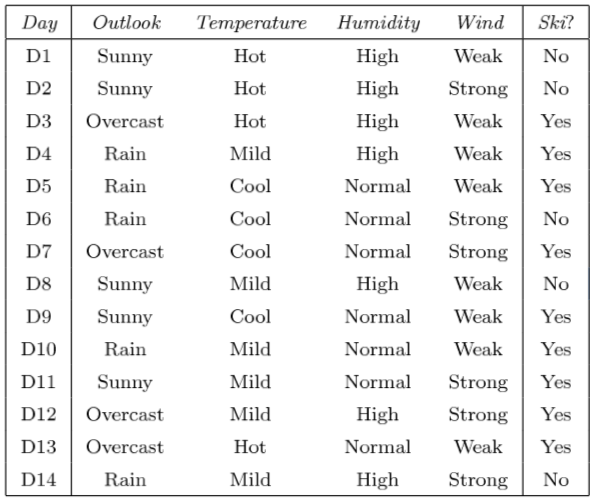
\includegraphics[scale=0.5]{img/dataset.png}
				\caption{A skiing example from \cite{cornell}}
			\end{figure}

			\noindent {\bf Output:}
			\begin{multicols}{2}
			\begin{table}[H]
					\begin{tabular}{rl}
					D: & ski(X) $\leftarrow$ member(X, [d4]). \\
					   & ski(X) $\leftarrow$ high(X), \textbackslash{+ab10(X)}. \\
					   & ski(X) $\leftarrow$ mild(X), \textbackslash{+ab1(X)}. \\
					   & ski(X) $\leftarrow$ normal(X),\textbackslash{+ab0(X)}. \\
					   & ski(X) $\leftarrow$ overcast(X). \\
					\end{tabular}
			\end{table}
			\columnbreak
			\begin{table}[H]
					\begin{tabular}{rl}
					AB:& ab0(X) $\leftarrow$ strong(X).\\
					   & ab1(X) $\leftarrow$ rain(X). \\
					   & ab1(X) $\leftarrow$ weak(X). \\
					   & ab10(X) $\leftarrow$ high(X). \\
					   & ab10(X) $\leftarrow$ sunny(X). \\
					\end{tabular}
			\end{table}
			\end{multicols}
		\end{subsection}
	\end{section}
	\begin{section}{Modification}
		Based on the steps of algorithms in the paper, I somehow modified some parts of the algorithm for the original one did not work when running the testing data. Perhaps the authors made some typos in the paper.

		First, in my code, the specialize function does not stop at IG=0. Instead, I changed the condition to -1. The reason is that if $n_0=0$ and $p_1 > 0$ after we found a rule $L+R$, the value of IG would be $log_2{1}-log_2{1}=0$, but actually we do not expect to go to exception function in this round for we had found a rule governing some positive examples. To fix this problem, only until there is no rule covering a subset of $E+$ do we turn to exception function, and we use -1 as the signal of it.

		Second, in line 27 of the FOLD psuedo code, the algorithm updates $E-$ at the end of every iteration in the specialize function. It eliminates the examples covered by the given clause. However, the uncovered examples should be removed, not the covered ones. Only leaving the covered examples can help us know if there exists an exception. Thus, I designed two functions, \emph{covered\_examples}/3 and \emph{uncovered\_examples}/3, to handle two different requests.

	\end{section}
	\begin{section}{Conclusion}
		In the previous first three tests, we can see that the algorithm successfully learned the theories of the dataset without the influnce of the noisy data or the exceptions. However, when the background knowledge becomes complicated like the skiing example, the algorithm caused some mistakes (2 out of 14) when we try to verify the knowledge with the generated rules. Besides, there are still some drawbacks in my implementation, such as the clauses high(X) and \textbackslash{+high(X)} exist at the same body, which is a contradiction and will always return false.
	\end{section}

	\begin{thebibliography}{unsrt}
		\bibitem{FOLD} Farhad Shakerin, Elmer Salazar, and Gopal Gupta, \textit{A New Algorithm to Automate Inductive Learning of Default Theories}, International Conference on Logic Programming (ICLP), Melbourne, 2017.
		\bibitem{cornell} Thorsten Joachims, CS478 - Machine Learning, Cornell University, Spring 2008. \textit{$<$http://www.cs.cornell.edu/courses/cs478/2000SP/lectures/rule-learning.pdf$>$}
	\end{thebibliography}
\end{document}